\documentclass[1p]{elsarticle_modified}
%\bibliographystyle{elsarticle-num}

%\usepackage[colorlinks]{hyperref}
%\usepackage{abbrmath_seonhwa} %\Abb, \Ascr, \Acal ,\Abf, \Afrak
\usepackage{amsfonts}
\usepackage{amssymb}
\usepackage{amsmath}
\usepackage{amsthm}
\usepackage{scalefnt}
\usepackage{amsbsy}
\usepackage{kotex}
\usepackage{caption}
\usepackage{subfig}
\usepackage{color}
\usepackage{graphicx}
\usepackage{xcolor} %% white, black, red, green, blue, cyan, magenta, yellow
\usepackage{float}
\usepackage{setspace}
\usepackage{hyperref}

\usepackage{tikz}
\usetikzlibrary{arrows}

\usepackage{multirow}
\usepackage{array} % fixed length table
\usepackage{hhline}

%%%%%%%%%%%%%%%%%%%%%
\makeatletter
\renewcommand*\env@matrix[1][\arraystretch]{%
	\edef\arraystretch{#1}%
	\hskip -\arraycolsep
	\let\@ifnextchar\new@ifnextchar
	\array{*\c@MaxMatrixCols c}}
\makeatother %https://tex.stackexchange.com/questions/14071/how-can-i-increase-the-line-spacing-in-a-matrix
%%%%%%%%%%%%%%%

\usepackage[normalem]{ulem}

\newcommand{\msout}[1]{\ifmmode\text{\sout{\ensuremath{#1}}}\else\sout{#1}\fi}
%SOURCE: \msout is \stkout macro in https://tex.stackexchange.com/questions/20609/strikeout-in-math-mode

\newcommand{\cancel}[1]{
	\ifmmode
	{\color{red}\msout{#1}}
	\else
	{\color{red}\sout{#1}}
	\fi
}

\newcommand{\add}[1]{
	{\color{blue}\uwave{#1}}
}

\newcommand{\replace}[2]{
	\ifmmode
	{\color{red}\msout{#1}}{\color{blue}\uwave{#2}}
	\else
	{\color{red}\sout{#1}}{\color{blue}\uwave{#2}}
	\fi
}

\newcommand{\Sol}{\mathcal{S}} %segment
\newcommand{\D}{D} %diagram
\newcommand{\A}{\mathcal{A}} %arc


%%%%%%%%%%%%%%%%%%%%%%%%%%%%%5 test

\def\sl{\operatorname{\textup{SL}}(2,\Cbb)}
\def\psl{\operatorname{\textup{PSL}}(2,\Cbb)}
\def\quan{\mkern 1mu \triangleright \mkern 1mu}

\theoremstyle{definition}
\newtheorem{thm}{Theorem}[section]
\newtheorem{prop}[thm]{Proposition}
\newtheorem{lem}[thm]{Lemma}
\newtheorem{ques}[thm]{Question}
\newtheorem{cor}[thm]{Corollary}
\newtheorem{defn}[thm]{Definition}
\newtheorem{exam}[thm]{Example}
\newtheorem{rmk}[thm]{Remark}
\newtheorem{alg}[thm]{Algorithm}

\newcommand{\I}{\sqrt{-1}}
\begin{document}

%\begin{frontmatter}
%
%\title{Boundary parabolic representations of knots up to 8 crossings}
%
%%% Group authors per affiliation:
%\author{Yunhi Cho} 
%\address{Department of Mathematics, University of Seoul, Seoul, Korea}
%\ead{yhcho@uos.ac.kr}
%
%
%\author{Seonhwa Kim} %\fnref{s_kim}}
%\address{Center for Geometry and Physics, Institute for Basic Science, Pohang, 37673, Korea}
%\ead{ryeona17@ibs.re.kr}
%
%\author{Hyuk Kim}
%\address{Department of Mathematical Sciences, Seoul National University, Seoul 08826, Korea}
%\ead{hyukkim@snu.ac.kr}
%
%\author{Seokbeom Yoon}
%\address{Department of Mathematical Sciences, Seoul National University, Seoul, 08826,  Korea}
%\ead{sbyoon15@snu.ac.kr}
%
%\begin{abstract}
%We find all boundary parabolic representation of knots up to 8 crossings.
%
%\end{abstract}
%\begin{keyword}
%    \MSC[2010] 57M25 
%\end{keyword}
%
%\end{frontmatter}

%\linenumbers
%\tableofcontents
%
\newcommand\colored[1]{\textcolor{white}{\rule[-0.35ex]{0.8em}{1.4ex}}\kern-0.8em\color{red} #1}%
%\newcommand\colored[1]{\textcolor{white}{ #1}\kern-2.17ex	\textcolor{white}{ #1}\kern-1.81ex	\textcolor{white}{ #1}\kern-2.15ex\color{red}#1	}

{\Large $\underline{12a_{0769}~(K12a_{0769})}$}

\setlength{\tabcolsep}{10pt}
\renewcommand{\arraystretch}{1.6}
\vspace{1cm}\begin{tabular}{m{100pt}>{\centering\arraybackslash}m{274pt}}
\multirow{5}{120pt}{
	\centering
	\includegraphics[width=112pt]{../../../GIT/diagram.site/Diagrams/png/1570_12a_0769.png}\\
\ \ \ A knot diagram\footnotemark}&
\allowdisplaybreaks
\textbf{Linearized knot diagam} \\
\cline{2-2}
 &
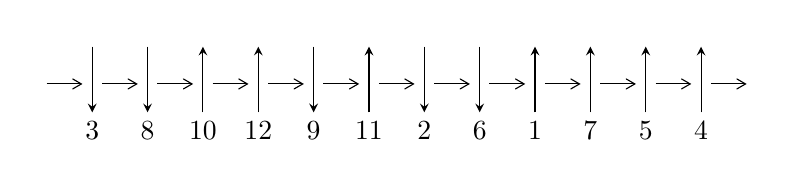
\begin{tikzpicture}[x=20pt, y=17pt]
	% nodes
	\node (C0) at (0, 0) {};
	\node (C1) at (1, 0) {};
	\node (C1U) at (1, +1) {};
	\node (C1D) at (1, -1) {3};

	\node (C2) at (2, 0) {};
	\node (C2U) at (2, +1) {};
	\node (C2D) at (2, -1) {8};

	\node (C3) at (3, 0) {};
	\node (C3U) at (3, +1) {};
	\node (C3D) at (3, -1) {10};

	\node (C4) at (4, 0) {};
	\node (C4U) at (4, +1) {};
	\node (C4D) at (4, -1) {12};

	\node (C5) at (5, 0) {};
	\node (C5U) at (5, +1) {};
	\node (C5D) at (5, -1) {9};

	\node (C6) at (6, 0) {};
	\node (C6U) at (6, +1) {};
	\node (C6D) at (6, -1) {11};

	\node (C7) at (7, 0) {};
	\node (C7U) at (7, +1) {};
	\node (C7D) at (7, -1) {2};

	\node (C8) at (8, 0) {};
	\node (C8U) at (8, +1) {};
	\node (C8D) at (8, -1) {6};

	\node (C9) at (9, 0) {};
	\node (C9U) at (9, +1) {};
	\node (C9D) at (9, -1) {1};

	\node (C10) at (10, 0) {};
	\node (C10U) at (10, +1) {};
	\node (C10D) at (10, -1) {7};

	\node (C11) at (11, 0) {};
	\node (C11U) at (11, +1) {};
	\node (C11D) at (11, -1) {5};

	\node (C12) at (12, 0) {};
	\node (C12U) at (12, +1) {};
	\node (C12D) at (12, -1) {4};
	\node (C13) at (13, 0) {};

	% arrows
	\draw[->,>={angle 60}]
	(C0) edge (C1) (C1) edge (C2) (C2) edge (C3) (C3) edge (C4) (C4) edge (C5) (C5) edge (C6) (C6) edge (C7) (C7) edge (C8) (C8) edge (C9) (C9) edge (C10) (C10) edge (C11) (C11) edge (C12) (C12) edge (C13) ;	\draw[->,>=stealth]
	(C1U) edge (C1D) (C2U) edge (C2D) (C3D) edge (C3U) (C4D) edge (C4U) (C5U) edge (C5D) (C6D) edge (C6U) (C7U) edge (C7D) (C8U) edge (C8D) (C9D) edge (C9U) (C10D) edge (C10U) (C11D) edge (C11U) (C12D) edge (C12U) ;
	\end{tikzpicture} \\
\hhline{~~} \\& 
\textbf{Solving Sequence} \\ \cline{2-2} 
 &
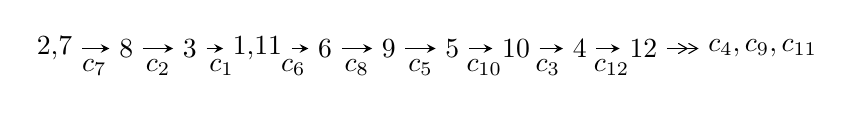
\begin{tikzpicture}[x=23pt, y=7pt]
	% node
	\node (A0) at (-1/8, 0) {2,7};
	\node (A1) at (1, 0) {8};
	\node (A2) at (2, 0) {3};
	\node (A3) at (49/16, 0) {1,11};
	\node (A4) at (33/8, 0) {6};
	\node (A5) at (41/8, 0) {9};
	\node (A6) at (49/8, 0) {5};
	\node (A7) at (57/8, 0) {10};
	\node (A8) at (65/8, 0) {4};
	\node (A9) at (73/8, 0) {12};
	\node (C1) at (1/2, -1) {$c_{7}$};
	\node (C2) at (3/2, -1) {$c_{2}$};
	\node (C3) at (5/2, -1) {$c_{1}$};
	\node (C4) at (29/8, -1) {$c_{6}$};
	\node (C5) at (37/8, -1) {$c_{8}$};
	\node (C6) at (45/8, -1) {$c_{5}$};
	\node (C7) at (53/8, -1) {$c_{10}$};
	\node (C8) at (61/8, -1) {$c_{3}$};
	\node (C9) at (69/8, -1) {$c_{12}$};
	\node (A10) at (11, 0) {$c_{4},c_{9},c_{11}$};

	% edge
	\draw[->,>=stealth]	
	(A0) edge (A1) (A1) edge (A2) (A2) edge (A3) (A3) edge (A4) (A4) edge (A5) (A5) edge (A6) (A6) edge (A7) (A7) edge (A8) (A8) edge (A9) ;
	\draw[->>,>={angle 60}]	
	(A9) edge (A10);
\end{tikzpicture} \\ 

\end{tabular} \\

\footnotetext{
The image of knot diagram is generated by the software ``\textbf{Draw programme}" developed by Andrew Bartholomew(\url{http://www.layer8.co.uk/maths/draw/index.htm\#Running-draw}), where we modified some parts for our purpose(\url{https://github.com/CATsTAILs/LinksPainter}).
}\phantom \\ \newline 
\centering \textbf{Ideals for irreducible components\footnotemark of $X_{\text{par}}$} 
 
\begin{align*}
I^u_{1}&=\langle 
4.90028\times10^{221} u^{119}-6.36136\times10^{221} u^{118}+\cdots+3.32809\times10^{221} b-7.62938\times10^{223},\\
\phantom{I^u_{1}}&\phantom{= \langle  }6.58487\times10^{222} u^{119}-1.43090\times10^{222} u^{118}+\cdots+1.05389\times10^{222} a-5.06564\times10^{224},\\
\phantom{I^u_{1}}&\phantom{= \langle  }u^{120}- u^{119}+\cdots-55 u+76\rangle \\
I^u_{2}&=\langle 
43 u^{25}+128 u^{24}+\cdots+49 b-207,\;235 u^{25}+246 u^{24}+\cdots+49 a-443,\;u^{26}-5 u^{24}+\cdots-6 u^2+1\rangle \\
\\
\end{align*}
\raggedright * 2 irreducible components of $\dim_{\mathbb{C}}=0$, with total 146 representations.\\
\footnotetext{All coefficients of polynomials are rational numbers. But the coefficients are sometimes approximated in decimal forms when there is not enough margin.}
\newpage
\renewcommand{\arraystretch}{1}
\centering \section*{I. $I^u_{1}= \langle 4.90\times10^{221} u^{119}-6.36\times10^{221} u^{118}+\cdots+3.33\times10^{221} b-7.63\times10^{223},\;6.58\times10^{222} u^{119}-1.43\times10^{222} u^{118}+\cdots+1.05\times10^{222} a-5.07\times10^{224},\;u^{120}- u^{119}+\cdots-55 u+76 \rangle$}
\flushleft \textbf{(i) Arc colorings}\\
\begin{tabular}{m{7pt} m{180pt} m{7pt} m{180pt} }
\flushright $a_{2}=$&$\begin{pmatrix}0\\u\end{pmatrix}$ \\
\flushright $a_{7}=$&$\begin{pmatrix}1\\0\end{pmatrix}$ \\
\flushright $a_{8}=$&$\begin{pmatrix}1\\u^2\end{pmatrix}$ \\
\flushright $a_{3}=$&$\begin{pmatrix}- u\\- u^3+u\end{pmatrix}$ \\
\flushright $a_{1}=$&$\begin{pmatrix}u^3\\u^5- u^3+u\end{pmatrix}$ \\
\flushright $a_{11}=$&$\begin{pmatrix}-6.24813 u^{119}+1.35773 u^{118}+\cdots+43.1116 u+480.660\\-1.47240 u^{119}+1.91142 u^{118}+\cdots+144.938 u+229.242\end{pmatrix}$ \\
\flushright $a_{6}=$&$\begin{pmatrix}-5.70471 u^{119}-0.638481 u^{118}+\cdots-97.4784 u+319.351\\-4.92763 u^{119}+0.244041 u^{118}+\cdots-31.4329 u+326.770\end{pmatrix}$ \\
\flushright $a_{9}=$&$\begin{pmatrix}-7.17248 u^{119}+1.42733 u^{118}+\cdots+47.5668 u+545.642\\-2.50902 u^{119}+2.36297 u^{118}+\cdots+177.669 u+326.769\end{pmatrix}$ \\
\flushright $a_{5}=$&$\begin{pmatrix}-7.55899 u^{119}-0.806060 u^{118}+\cdots-153.369 u+406.441\\-4.70727 u^{119}+0.223186 u^{118}+\cdots-30.9319 u+305.682\end{pmatrix}$ \\
\flushright $a_{10}=$&$\begin{pmatrix}-4.77573 u^{119}-0.553687 u^{118}+\cdots-101.826 u+251.418\\-1.47240 u^{119}+1.91142 u^{118}+\cdots+144.938 u+229.242\end{pmatrix}$ \\
\flushright $a_{4}=$&$\begin{pmatrix}-6.42549 u^{119}-0.253055 u^{118}+\cdots-48.4915 u+394.825\\-3.76726 u^{119}+0.426794 u^{118}+\cdots+2.87528 u+263.024\end{pmatrix}$ \\
\flushright $a_{12}=$&$\begin{pmatrix}4.90188 u^{119}-3.66164 u^{118}+\cdots-345.185 u-620.459\\0.318017 u^{119}-1.90163 u^{118}+\cdots-189.757 u-184.421\end{pmatrix}$\\&\end{tabular}
\flushleft \textbf{(ii) Obstruction class $= -1$}\\~\\
\flushleft \textbf{(iii) Cusp Shapes $= 11.9826 u^{119}-3.58926 u^{118}+\cdots-186.522 u-990.154$}\\~\\
\newpage\renewcommand{\arraystretch}{1}
\flushleft \textbf{(iv) u-Polynomials at the component}\newline \\
\begin{tabular}{m{50pt}|m{274pt}}
Crossings & \hspace{64pt}u-Polynomials at each crossing \\
\hline $$\begin{aligned}c_{1}\end{aligned}$$&$\begin{aligned}
&u^{120}+49 u^{119}+\cdots+96657 u+5776
\end{aligned}$\\
\hline $$\begin{aligned}c_{2},c_{7}\end{aligned}$$&$\begin{aligned}
&u^{120}+u^{119}+\cdots+55 u+76
\end{aligned}$\\
\hline $$\begin{aligned}c_{3}\end{aligned}$$&$\begin{aligned}
&u^{120}+15 u^{118}+\cdots+8192 u+1024
\end{aligned}$\\
\hline $$\begin{aligned}c_{4},c_{11},c_{12}\end{aligned}$$&$\begin{aligned}
&u^{120}+3 u^{119}+\cdots+u+2
\end{aligned}$\\
\hline $$\begin{aligned}c_{5},c_{8}\end{aligned}$$&$\begin{aligned}
&u^{120}-4 u^{119}+\cdots-288 u+112
\end{aligned}$\\
\hline $$\begin{aligned}c_{6},c_{10}\end{aligned}$$&$\begin{aligned}
&u^{120}- u^{119}+\cdots+10311 u+1766
\end{aligned}$\\
\hline $$\begin{aligned}c_{9}\end{aligned}$$&$\begin{aligned}
&u^{120}-7 u^{119}+\cdots+3752 u+928
\end{aligned}$\\
\hline
\end{tabular}\\~\\
\newpage\renewcommand{\arraystretch}{1}
\flushleft \textbf{(v) Riley Polynomials at the component}\newline \\
\begin{tabular}{m{50pt}|m{274pt}}
Crossings & \hspace{64pt}Riley Polynomials at each crossing \\
\hline $$\begin{aligned}c_{1}\end{aligned}$$&$\begin{aligned}
&y^{120}+43 y^{119}+\cdots+814266207 y+33362176
\end{aligned}$\\
\hline $$\begin{aligned}c_{2},c_{7}\end{aligned}$$&$\begin{aligned}
&y^{120}-49 y^{119}+\cdots-96657 y+5776
\end{aligned}$\\
\hline $$\begin{aligned}c_{3}\end{aligned}$$&$\begin{aligned}
&y^{120}+30 y^{119}+\cdots+22020096 y+1048576
\end{aligned}$\\
\hline $$\begin{aligned}c_{4},c_{11},c_{12}\end{aligned}$$&$\begin{aligned}
&y^{120}+123 y^{119}+\cdots+311 y+4
\end{aligned}$\\
\hline $$\begin{aligned}c_{5},c_{8}\end{aligned}$$&$\begin{aligned}
&y^{120}+68 y^{119}+\cdots+688512 y+12544
\end{aligned}$\\
\hline $$\begin{aligned}c_{6},c_{10}\end{aligned}$$&$\begin{aligned}
&y^{120}+83 y^{119}+\cdots+16685179 y+3118756
\end{aligned}$\\
\hline $$\begin{aligned}c_{9}\end{aligned}$$&$\begin{aligned}
&y^{120}+y^{119}+\cdots-8464960 y+861184
\end{aligned}$\\
\hline
\end{tabular}\\~\\
\newpage\flushleft \textbf{(vi) Complex Volumes and Cusp Shapes}
$$\begin{array}{c|c|c}  
\text{Solutions to }I^u_{1}& \I (\text{vol} + \sqrt{-1}CS) & \text{Cusp shape}\\
 \hline 
\begin{aligned}
u &= \phantom{-}0.640376 + 0.754506 I \\
a &= -0.273310 - 0.956734 I \\
b &= \phantom{-}1.042890 - 0.294443 I\end{aligned}
 & \phantom{-}5.13060 + 2.11657 I & \phantom{-0.000000 } 0 \\ \hline\begin{aligned}
u &= \phantom{-}0.640376 - 0.754506 I \\
a &= -0.273310 + 0.956734 I \\
b &= \phantom{-}1.042890 + 0.294443 I\end{aligned}
 & \phantom{-}5.13060 - 2.11657 I & \phantom{-0.000000 } 0 \\ \hline\begin{aligned}
u &= -0.526278 + 0.835444 I \\
a &= \phantom{-}0.404937 - 0.002448 I \\
b &= -0.290883 + 1.201140 I\end{aligned}
 & -7.92215 - 4.97148 I & \phantom{-0.000000 } 0 \\ \hline\begin{aligned}
u &= -0.526278 - 0.835444 I \\
a &= \phantom{-}0.404937 + 0.002448 I \\
b &= -0.290883 - 1.201140 I\end{aligned}
 & -7.92215 + 4.97148 I & \phantom{-0.000000 } 0 \\ \hline\begin{aligned}
u &= \phantom{-}0.882437 + 0.436290 I \\
a &= -1.72646 - 2.00320 I \\
b &= -0.14486 - 2.24214 I\end{aligned}
 & -10.71680 - 1.79302 I & \phantom{-0.000000 } 0 \\ \hline\begin{aligned}
u &= \phantom{-}0.882437 - 0.436290 I \\
a &= -1.72646 + 2.00320 I \\
b &= -0.14486 + 2.24214 I\end{aligned}
 & -10.71680 + 1.79302 I & \phantom{-0.000000 } 0 \\ \hline\begin{aligned}
u &= -0.895202 + 0.495352 I \\
a &= -0.94608 + 2.31227 I \\
b &= \phantom{-}0.087800 + 1.396210 I\end{aligned}
 & -1.78369 + 2.17868 I & \phantom{-0.000000 } 0 \\ \hline\begin{aligned}
u &= -0.895202 - 0.495352 I \\
a &= -0.94608 - 2.31227 I \\
b &= \phantom{-}0.087800 - 1.396210 I\end{aligned}
 & -1.78369 - 2.17868 I & \phantom{-0.000000 } 0 \\ \hline\begin{aligned}
u &= \phantom{-}0.914841 + 0.478429 I \\
a &= \phantom{-}1.52846 + 1.20791 I \\
b &= -0.378324 + 1.071270 I\end{aligned}
 & -1.78722 - 2.37288 I & \phantom{-0.000000 } 0 \\ \hline\begin{aligned}
u &= \phantom{-}0.914841 - 0.478429 I \\
a &= \phantom{-}1.52846 - 1.20791 I \\
b &= -0.378324 - 1.071270 I\end{aligned}
 & -1.78722 + 2.37288 I & \phantom{-0.000000 } 0\\
 \hline 
 \end{array}$$\newpage$$\begin{array}{c|c|c}  
\text{Solutions to }I^u_{1}& \I (\text{vol} + \sqrt{-1}CS) & \text{Cusp shape}\\
 \hline 
\begin{aligned}
u &= -0.832669 + 0.489433 I \\
a &= -0.35939 + 1.69937 I \\
b &= -0.358930 + 1.273050 I\end{aligned}
 & -1.56898 + 1.83315 I & \phantom{-0.000000 } 0 \\ \hline\begin{aligned}
u &= -0.832669 - 0.489433 I \\
a &= -0.35939 - 1.69937 I \\
b &= -0.358930 - 1.273050 I\end{aligned}
 & -1.56898 - 1.83315 I & \phantom{-0.000000 } 0 \\ \hline\begin{aligned}
u &= \phantom{-}0.883036 + 0.381686 I \\
a &= \phantom{-}0.189734 + 0.020446 I \\
b &= \phantom{-}0.499406 + 0.462228 I\end{aligned}
 & -1.35072 - 1.18683 I & \phantom{-0.000000 } 0 \\ \hline\begin{aligned}
u &= \phantom{-}0.883036 - 0.381686 I \\
a &= \phantom{-}0.189734 - 0.020446 I \\
b &= \phantom{-}0.499406 - 0.462228 I\end{aligned}
 & -1.35072 + 1.18683 I & \phantom{-0.000000 } 0 \\ \hline\begin{aligned}
u &= \phantom{-}0.809652 + 0.656870 I \\
a &= \phantom{-}0.848716 + 0.218807 I \\
b &= -0.720338 + 0.598197 I\end{aligned}
 & -1.31759 - 1.23542 I & \phantom{-0.000000 } 0 \\ \hline\begin{aligned}
u &= \phantom{-}0.809652 - 0.656870 I \\
a &= \phantom{-}0.848716 - 0.218807 I \\
b &= -0.720338 - 0.598197 I\end{aligned}
 & -1.31759 + 1.23542 I & \phantom{-0.000000 } 0 \\ \hline\begin{aligned}
u &= -0.872320 + 0.393222 I \\
a &= \phantom{-}2.21646 - 1.59565 I \\
b &= -0.065607 - 0.821017 I\end{aligned}
 & \phantom{-}0.041033 - 0.859294 I & \phantom{-0.000000 } 0 \\ \hline\begin{aligned}
u &= -0.872320 - 0.393222 I \\
a &= \phantom{-}2.21646 + 1.59565 I \\
b &= -0.065607 + 0.821017 I\end{aligned}
 & \phantom{-}0.041033 + 0.859294 I & \phantom{-0.000000 } 0 \\ \hline\begin{aligned}
u &= -1.034920 + 0.226485 I \\
a &= \phantom{-}0.853083 - 0.590111 I \\
b &= \phantom{-}0.801681 - 0.687458 I\end{aligned}
 & -6.96211 + 0.05806 I & \phantom{-0.000000 } 0 \\ \hline\begin{aligned}
u &= -1.034920 - 0.226485 I \\
a &= \phantom{-}0.853083 + 0.590111 I \\
b &= \phantom{-}0.801681 + 0.687458 I\end{aligned}
 & -6.96211 - 0.05806 I & \phantom{-0.000000 } 0\\
 \hline 
 \end{array}$$\newpage$$\begin{array}{c|c|c}  
\text{Solutions to }I^u_{1}& \I (\text{vol} + \sqrt{-1}CS) & \text{Cusp shape}\\
 \hline 
\begin{aligned}
u &= \phantom{-}0.472677 + 0.954639 I \\
a &= -0.039591 + 0.315286 I \\
b &= \phantom{-}0.66236 + 1.30816 I\end{aligned}
 & -4.59021 + 12.29690 I & \phantom{-0.000000 } 0 \\ \hline\begin{aligned}
u &= \phantom{-}0.472677 - 0.954639 I \\
a &= -0.039591 - 0.315286 I \\
b &= \phantom{-}0.66236 - 1.30816 I\end{aligned}
 & -4.59021 - 12.29690 I & \phantom{-0.000000 } 0 \\ \hline\begin{aligned}
u &= -0.695176 + 0.610567 I \\
a &= \phantom{-}0.837440 + 0.424941 I \\
b &= -0.607307 + 0.978322 I\end{aligned}
 & -2.45014 - 3.81871 I & \phantom{-0.000000 } 0 \\ \hline\begin{aligned}
u &= -0.695176 - 0.610567 I \\
a &= \phantom{-}0.837440 - 0.424941 I \\
b &= -0.607307 - 0.978322 I\end{aligned}
 & -2.45014 + 3.81871 I & \phantom{-0.000000 } 0 \\ \hline\begin{aligned}
u &= \phantom{-}0.937857 + 0.536832 I \\
a &= -1.29364 - 2.46504 I \\
b &= \phantom{-}0.381221 - 1.189800 I\end{aligned}
 & \phantom{-}1.04041 - 5.59127 I & \phantom{-0.000000 } 0 \\ \hline\begin{aligned}
u &= \phantom{-}0.937857 - 0.536832 I \\
a &= -1.29364 + 2.46504 I \\
b &= \phantom{-}0.381221 + 1.189800 I\end{aligned}
 & \phantom{-}1.04041 + 5.59127 I & \phantom{-0.000000 } 0 \\ \hline\begin{aligned}
u &= -0.466942 + 0.975547 I \\
a &= \phantom{-}0.032907 - 0.446919 I \\
b &= \phantom{-}0.580562 - 1.221380 I\end{aligned}
 & \phantom{-}2.18598 - 7.87003 I & \phantom{-0.000000 } 0 \\ \hline\begin{aligned}
u &= -0.466942 - 0.975547 I \\
a &= \phantom{-}0.032907 + 0.446919 I \\
b &= \phantom{-}0.580562 + 1.221380 I\end{aligned}
 & \phantom{-}2.18598 + 7.87003 I & \phantom{-0.000000 } 0 \\ \hline\begin{aligned}
u &= -0.972631 + 0.474931 I \\
a &= -0.478168 + 0.389429 I \\
b &= \phantom{-}0.495723 - 0.238417 I\end{aligned}
 & -0.55152 + 4.16383 I & \phantom{-0.000000 } 0 \\ \hline\begin{aligned}
u &= -0.972631 - 0.474931 I \\
a &= -0.478168 - 0.389429 I \\
b &= \phantom{-}0.495723 + 0.238417 I\end{aligned}
 & -0.55152 - 4.16383 I & \phantom{-0.000000 } 0\\
 \hline 
 \end{array}$$\newpage$$\begin{array}{c|c|c}  
\text{Solutions to }I^u_{1}& \I (\text{vol} + \sqrt{-1}CS) & \text{Cusp shape}\\
 \hline 
\begin{aligned}
u &= \phantom{-}0.845008 + 0.351940 I \\
a &= \phantom{-}2.45288 + 2.44208 I \\
b &= \phantom{-}0.111293 + 0.735777 I\end{aligned}
 & -4.95807 + 3.90695 I & \phantom{-0.000000 } 0 \\ \hline\begin{aligned}
u &= \phantom{-}0.845008 - 0.351940 I \\
a &= \phantom{-}2.45288 - 2.44208 I \\
b &= \phantom{-}0.111293 - 0.735777 I\end{aligned}
 & -4.95807 - 3.90695 I & \phantom{-0.000000 } 0 \\ \hline\begin{aligned}
u &= -0.578766 + 0.699373 I \\
a &= -0.472636 + 1.200260 I \\
b &= \phantom{-}1.290760 + 0.327675 I\end{aligned}
 & -1.33795 - 5.57386 I & \phantom{-0.000000 } 0 \\ \hline\begin{aligned}
u &= -0.578766 - 0.699373 I \\
a &= -0.472636 - 1.200260 I \\
b &= \phantom{-}1.290760 - 0.327675 I\end{aligned}
 & -1.33795 + 5.57386 I & \phantom{-0.000000 } 0 \\ \hline\begin{aligned}
u &= \phantom{-}0.886943 + 0.175895 I \\
a &= -0.613692 + 0.718318 I \\
b &= -1.198730 - 0.548916 I\end{aligned}
 & -5.60557 + 5.04751 I & \phantom{-0.000000 } 0 \\ \hline\begin{aligned}
u &= \phantom{-}0.886943 - 0.175895 I \\
a &= -0.613692 - 0.718318 I \\
b &= -1.198730 + 0.548916 I\end{aligned}
 & -5.60557 - 5.04751 I & \phantom{-0.000000 } 0 \\ \hline\begin{aligned}
u &= \phantom{-}0.739706 + 0.509645 I \\
a &= \phantom{-}0.332396 - 0.867037 I \\
b &= -0.575450 - 1.044550 I\end{aligned}
 & \phantom{-}1.69152 + 1.31290 I & \phantom{-0.000000 } 0 \\ \hline\begin{aligned}
u &= \phantom{-}0.739706 - 0.509645 I \\
a &= \phantom{-}0.332396 + 0.867037 I \\
b &= -0.575450 + 1.044550 I\end{aligned}
 & \phantom{-}1.69152 - 1.31290 I & \phantom{-0.000000 } 0 \\ \hline\begin{aligned}
u &= -0.747119 + 0.815803 I \\
a &= -0.086094 + 0.707533 I \\
b &= \phantom{-}0.621373 + 0.213296 I\end{aligned}
 & \phantom{-}4.69145 + 2.28641 I & \phantom{-0.000000 } 0 \\ \hline\begin{aligned}
u &= -0.747119 - 0.815803 I \\
a &= -0.086094 - 0.707533 I \\
b &= \phantom{-}0.621373 - 0.213296 I\end{aligned}
 & \phantom{-}4.69145 - 2.28641 I & \phantom{-0.000000 } 0\\
 \hline 
 \end{array}$$\newpage$$\begin{array}{c|c|c}  
\text{Solutions to }I^u_{1}& \I (\text{vol} + \sqrt{-1}CS) & \text{Cusp shape}\\
 \hline 
\begin{aligned}
u &= \phantom{-}1.015460 + 0.447308 I \\
a &= -1.317700 - 0.432286 I \\
b &= \phantom{-}0.237227 + 0.107181 I\end{aligned}
 & -5.79389 - 7.01675 I & \phantom{-0.000000 } 0 \\ \hline\begin{aligned}
u &= \phantom{-}1.015460 - 0.447308 I \\
a &= -1.317700 + 0.432286 I \\
b &= \phantom{-}0.237227 - 0.107181 I\end{aligned}
 & -5.79389 + 7.01675 I & \phantom{-0.000000 } 0 \\ \hline\begin{aligned}
u &= \phantom{-}0.455745 + 0.753757 I \\
a &= \phantom{-}0.508301 - 0.127039 I \\
b &= -0.326725 - 0.980508 I\end{aligned}
 & -1.21124 + 2.82506 I & \phantom{-0.000000 } 0 \\ \hline\begin{aligned}
u &= \phantom{-}0.455745 - 0.753757 I \\
a &= \phantom{-}0.508301 + 0.127039 I \\
b &= -0.326725 + 0.980508 I\end{aligned}
 & -1.21124 - 2.82506 I & \phantom{-0.000000 } 0 \\ \hline\begin{aligned}
u &= \phantom{-}1.070650 + 0.334394 I \\
a &= \phantom{-}1.11732 + 1.32635 I \\
b &= \phantom{-}0.442128 + 1.240410 I\end{aligned}
 & -2.93359 - 0.36031 I & \phantom{-0.000000 } 0 \\ \hline\begin{aligned}
u &= \phantom{-}1.070650 - 0.334394 I \\
a &= \phantom{-}1.11732 - 1.32635 I \\
b &= \phantom{-}0.442128 - 1.240410 I\end{aligned}
 & -2.93359 + 0.36031 I & \phantom{-0.000000 } 0 \\ \hline\begin{aligned}
u &= -0.958174 + 0.583219 I \\
a &= -1.68183 + 2.25035 I \\
b &= \phantom{-}0.511496 + 1.072450 I\end{aligned}
 & -3.26276 + 8.54514 I & \phantom{-0.000000 } 0 \\ \hline\begin{aligned}
u &= -0.958174 - 0.583219 I \\
a &= -1.68183 - 2.25035 I \\
b &= \phantom{-}0.511496 - 1.072450 I\end{aligned}
 & -3.26276 - 8.54514 I & \phantom{-0.000000 } 0 \\ \hline\begin{aligned}
u &= -0.988511 + 0.551859 I \\
a &= \phantom{-}1.36500 - 1.43555 I \\
b &= -0.47857 - 1.64419 I\end{aligned}
 & -9.67224 + 2.94134 I & \phantom{-0.000000 } 0 \\ \hline\begin{aligned}
u &= -0.988511 - 0.551859 I \\
a &= \phantom{-}1.36500 + 1.43555 I \\
b &= -0.47857 + 1.64419 I\end{aligned}
 & -9.67224 - 2.94134 I & \phantom{-0.000000 } 0\\
 \hline 
 \end{array}$$\newpage$$\begin{array}{c|c|c}  
\text{Solutions to }I^u_{1}& \I (\text{vol} + \sqrt{-1}CS) & \text{Cusp shape}\\
 \hline 
\begin{aligned}
u &= \phantom{-}0.885154 + 0.709753 I \\
a &= \phantom{-}0.272074 - 0.779465 I \\
b &= \phantom{-}0.640083 + 0.500521 I\end{aligned}
 & -1.51750 - 4.05330 I & \phantom{-0.000000 } 0 \\ \hline\begin{aligned}
u &= \phantom{-}0.885154 - 0.709753 I \\
a &= \phantom{-}0.272074 + 0.779465 I \\
b &= \phantom{-}0.640083 - 0.500521 I\end{aligned}
 & -1.51750 + 4.05330 I & \phantom{-0.000000 } 0 \\ \hline\begin{aligned}
u &= -0.150218 + 1.125420 I \\
a &= \phantom{-}0.234940 + 0.606687 I \\
b &= \phantom{-}0.177560 + 0.897894 I\end{aligned}
 & \phantom{-}1.59223 + 0.82756 I & \phantom{-0.000000 } 0 \\ \hline\begin{aligned}
u &= -0.150218 - 1.125420 I \\
a &= \phantom{-}0.234940 - 0.606687 I \\
b &= \phantom{-}0.177560 - 0.897894 I\end{aligned}
 & \phantom{-}1.59223 - 0.82756 I & \phantom{-0.000000 } 0 \\ \hline\begin{aligned}
u &= -0.478342 + 0.702792 I \\
a &= \phantom{-}0.559900 + 0.148553 I \\
b &= \phantom{-}0.205940 - 1.327080 I\end{aligned}
 & -8.23370 + 1.80575 I & \phantom{-0.000000 } 0 \\ \hline\begin{aligned}
u &= -0.478342 - 0.702792 I \\
a &= \phantom{-}0.559900 - 0.148553 I \\
b &= \phantom{-}0.205940 + 1.327080 I\end{aligned}
 & -8.23370 - 1.80575 I & \phantom{-0.000000 } 0 \\ \hline\begin{aligned}
u &= \phantom{-}1.162960 + 0.015963 I \\
a &= -0.17549 + 2.26357 I \\
b &= \phantom{-}0.16472 + 1.48066 I\end{aligned}
 & -13.9002 + 3.2371 I & \phantom{-0.000000 } 0 \\ \hline\begin{aligned}
u &= \phantom{-}1.162960 - 0.015963 I \\
a &= -0.17549 - 2.26357 I \\
b &= \phantom{-}0.16472 - 1.48066 I\end{aligned}
 & -13.9002 - 3.2371 I & \phantom{-0.000000 } 0 \\ \hline\begin{aligned}
u &= -0.878585 + 0.772283 I \\
a &= \phantom{-}0.365079 + 0.400564 I \\
b &= -0.041316 - 0.479766 I\end{aligned}
 & \phantom{-}4.22944 + 2.91051 I & \phantom{-0.000000 } 0 \\ \hline\begin{aligned}
u &= -0.878585 - 0.772283 I \\
a &= \phantom{-}0.365079 - 0.400564 I \\
b &= -0.041316 + 0.479766 I\end{aligned}
 & \phantom{-}4.22944 - 2.91051 I & \phantom{-0.000000 } 0\\
 \hline 
 \end{array}$$\newpage$$\begin{array}{c|c|c}  
\text{Solutions to }I^u_{1}& \I (\text{vol} + \sqrt{-1}CS) & \text{Cusp shape}\\
 \hline 
\begin{aligned}
u &= -1.120880 + 0.344185 I \\
a &= \phantom{-}0.07241 - 1.61285 I \\
b &= \phantom{-}0.108071 - 0.859897 I\end{aligned}
 & -6.25035 + 0.01892 I & \phantom{-0.000000 } 0 \\ \hline\begin{aligned}
u &= -1.120880 - 0.344185 I \\
a &= \phantom{-}0.07241 + 1.61285 I \\
b &= \phantom{-}0.108071 + 0.859897 I\end{aligned}
 & -6.25035 - 0.01892 I & \phantom{-0.000000 } 0 \\ \hline\begin{aligned}
u &= -1.117730 + 0.361741 I \\
a &= \phantom{-}1.32383 - 1.24388 I \\
b &= \phantom{-}0.53827 - 1.51484 I\end{aligned}
 & -8.26977 - 0.16688 I & \phantom{-0.000000 } 0 \\ \hline\begin{aligned}
u &= -1.117730 - 0.361741 I \\
a &= \phantom{-}1.32383 + 1.24388 I \\
b &= \phantom{-}0.53827 + 1.51484 I\end{aligned}
 & -8.26977 + 0.16688 I & \phantom{-0.000000 } 0 \\ \hline\begin{aligned}
u &= -1.061330 + 0.508158 I \\
a &= -0.89192 + 1.97682 I \\
b &= \phantom{-}0.85279 + 1.14210 I\end{aligned}
 & -1.81518 + 6.56693 I & \phantom{-0.000000 } 0 \\ \hline\begin{aligned}
u &= -1.061330 - 0.508158 I \\
a &= -0.89192 - 1.97682 I \\
b &= \phantom{-}0.85279 - 1.14210 I\end{aligned}
 & -1.81518 - 6.56693 I & \phantom{-0.000000 } 0 \\ \hline\begin{aligned}
u &= \phantom{-}1.082650 + 0.461042 I \\
a &= -0.72573 - 2.16920 I \\
b &= \phantom{-}1.03655 - 1.34819 I\end{aligned}
 & -7.66656 - 7.57137 I & \phantom{-0.000000 } 0 \\ \hline\begin{aligned}
u &= \phantom{-}1.082650 - 0.461042 I \\
a &= -0.72573 + 2.16920 I \\
b &= \phantom{-}1.03655 + 1.34819 I\end{aligned}
 & -7.66656 + 7.57137 I & \phantom{-0.000000 } 0 \\ \hline\begin{aligned}
u &= \phantom{-}0.874346 + 0.790463 I \\
a &= \phantom{-}0.615703 - 0.470871 I \\
b &= -0.078613 + 0.882615 I\end{aligned}
 & -0.00142 - 2.96056 I & \phantom{-0.000000 } 0 \\ \hline\begin{aligned}
u &= \phantom{-}0.874346 - 0.790463 I \\
a &= \phantom{-}0.615703 + 0.470871 I \\
b &= -0.078613 - 0.882615 I\end{aligned}
 & -0.00142 + 2.96056 I & \phantom{-0.000000 } 0\\
 \hline 
 \end{array}$$\newpage$$\begin{array}{c|c|c}  
\text{Solutions to }I^u_{1}& \I (\text{vol} + \sqrt{-1}CS) & \text{Cusp shape}\\
 \hline 
\begin{aligned}
u &= -0.947454 + 0.705336 I \\
a &= \phantom{-}0.050044 - 0.235893 I \\
b &= -0.756499 - 0.099528 I\end{aligned}
 & \phantom{-}4.04803 + 3.39775 I & \phantom{-0.000000 } 0 \\ \hline\begin{aligned}
u &= -0.947454 - 0.705336 I \\
a &= \phantom{-}0.050044 + 0.235893 I \\
b &= -0.756499 + 0.099528 I\end{aligned}
 & \phantom{-}4.04803 - 3.39775 I & \phantom{-0.000000 } 0 \\ \hline\begin{aligned}
u &= \phantom{-}0.510655 + 1.067890 I \\
a &= -0.020351 - 0.392987 I \\
b &= \phantom{-}0.263141 - 1.006270 I\end{aligned}
 & -4.23224 - 6.56669 I & \phantom{-0.000000 } 0 \\ \hline\begin{aligned}
u &= \phantom{-}0.510655 - 1.067890 I \\
a &= -0.020351 + 0.392987 I \\
b &= \phantom{-}0.263141 + 1.006270 I\end{aligned}
 & -4.23224 + 6.56669 I & \phantom{-0.000000 } 0 \\ \hline\begin{aligned}
u &= -1.024770 + 0.614403 I \\
a &= -0.543083 - 0.844425 I \\
b &= -1.55541 + 0.18806 I\end{aligned}
 & -2.67491 + 10.64940 I & \phantom{-0.000000 } 0 \\ \hline\begin{aligned}
u &= -1.024770 - 0.614403 I \\
a &= -0.543083 + 0.844425 I \\
b &= -1.55541 - 0.18806 I\end{aligned}
 & -2.67491 - 10.64940 I & \phantom{-0.000000 } 0 \\ \hline\begin{aligned}
u &= \phantom{-}1.004810 + 0.652032 I \\
a &= -0.325232 + 0.602839 I \\
b &= -1.225640 - 0.112802 I\end{aligned}
 & \phantom{-}4.01972 - 7.46198 I & \phantom{-0.000000 } 0 \\ \hline\begin{aligned}
u &= \phantom{-}1.004810 - 0.652032 I \\
a &= -0.325232 - 0.602839 I \\
b &= -1.225640 + 0.112802 I\end{aligned}
 & \phantom{-}4.01972 + 7.46198 I & \phantom{-0.000000 } 0 \\ \hline\begin{aligned}
u &= \phantom{-}0.489454 + 1.098110 I \\
a &= \phantom{-}0.226348 + 0.610901 I \\
b &= \phantom{-}0.376642 + 1.161960 I\end{aligned}
 & \phantom{-}1.92369 + 1.64383 I & \phantom{-0.000000 } 0 \\ \hline\begin{aligned}
u &= \phantom{-}0.489454 - 1.098110 I \\
a &= \phantom{-}0.226348 - 0.610901 I \\
b &= \phantom{-}0.376642 - 1.161960 I\end{aligned}
 & \phantom{-}1.92369 - 1.64383 I & \phantom{-0.000000 } 0\\
 \hline 
 \end{array}$$\newpage$$\begin{array}{c|c|c}  
\text{Solutions to }I^u_{1}& \I (\text{vol} + \sqrt{-1}CS) & \text{Cusp shape}\\
 \hline 
\begin{aligned}
u &= -1.203110 + 0.141860 I \\
a &= -0.01063 - 1.99891 I \\
b &= \phantom{-}0.047918 - 1.218620 I\end{aligned}
 & -6.29656 - 0.50343 I & \phantom{-0.000000 } 0 \\ \hline\begin{aligned}
u &= -1.203110 - 0.141860 I \\
a &= -0.01063 + 1.99891 I \\
b &= \phantom{-}0.047918 + 1.218620 I\end{aligned}
 & -6.29656 + 0.50343 I & \phantom{-0.000000 } 0 \\ \hline\begin{aligned}
u &= \phantom{-}1.088030 + 0.538755 I \\
a &= -0.62773 - 1.56135 I \\
b &= \phantom{-}0.931399 - 0.613542 I\end{aligned}
 & -5.08544 - 6.87789 I & \phantom{-0.000000 } 0 \\ \hline\begin{aligned}
u &= \phantom{-}1.088030 - 0.538755 I \\
a &= -0.62773 + 1.56135 I \\
b &= \phantom{-}0.931399 + 0.613542 I\end{aligned}
 & -5.08544 + 6.87789 I & \phantom{-0.000000 } 0 \\ \hline\begin{aligned}
u &= \phantom{-}0.679820 + 0.336957 I \\
a &= \phantom{-}1.232030 - 0.681094 I \\
b &= -0.406069 + 0.398167 I\end{aligned}
 & -1.81621 - 1.39548 I & \phantom{-0.000000 -}0. + 4.94228 I \\ \hline\begin{aligned}
u &= \phantom{-}0.679820 - 0.336957 I \\
a &= \phantom{-}1.232030 + 0.681094 I \\
b &= -0.406069 - 0.398167 I\end{aligned}
 & -1.81621 + 1.39548 I & \phantom{-0.000000 } 0. - 4.94228 I \\ \hline\begin{aligned}
u &= \phantom{-}1.088030 + 0.622795 I \\
a &= -1.35243 - 1.36217 I \\
b &= \phantom{-}0.445681 - 1.106640 I\end{aligned}
 & -3.05949 - 8.07209 I & \phantom{-0.000000 } 0 \\ \hline\begin{aligned}
u &= \phantom{-}1.088030 - 0.622795 I \\
a &= -1.35243 + 1.36217 I \\
b &= \phantom{-}0.445681 + 1.106640 I\end{aligned}
 & -3.05949 + 8.07209 I & \phantom{-0.000000 } 0 \\ \hline\begin{aligned}
u &= \phantom{-}0.337789 + 0.657214 I \\
a &= \phantom{-}0.819345 + 0.033021 I \\
b &= -0.839678 - 0.535416 I\end{aligned}
 & -2.95335 + 2.23609 I & \phantom{-}2.00000 - 1.76365 I \\ \hline\begin{aligned}
u &= \phantom{-}0.337789 - 0.657214 I \\
a &= \phantom{-}0.819345 - 0.033021 I \\
b &= -0.839678 + 0.535416 I\end{aligned}
 & -2.95335 - 2.23609 I & \phantom{-}2.00000 + 1.76365 I\\
 \hline 
 \end{array}$$\newpage$$\begin{array}{c|c|c}  
\text{Solutions to }I^u_{1}& \I (\text{vol} + \sqrt{-1}CS) & \text{Cusp shape}\\
 \hline 
\begin{aligned}
u &= -1.087990 + 0.666342 I \\
a &= -1.51101 + 1.19215 I \\
b &= \phantom{-}0.428378 + 1.252690 I\end{aligned}
 & -9.6150 + 10.5872 I & \phantom{-0.000000 } 0 \\ \hline\begin{aligned}
u &= -1.087990 - 0.666342 I \\
a &= -1.51101 - 1.19215 I \\
b &= \phantom{-}0.428378 - 1.252690 I\end{aligned}
 & -9.6150 - 10.5872 I & \phantom{-0.000000 } 0 \\ \hline\begin{aligned}
u &= -0.692575 + 0.103205 I \\
a &= -0.006438 - 0.545981 I \\
b &= -0.783820 + 0.630029 I\end{aligned}
 & \phantom{-}0.33138 - 2.81172 I & -1.59494 + 8.15444 I \\ \hline\begin{aligned}
u &= -0.692575 - 0.103205 I \\
a &= -0.006438 + 0.545981 I \\
b &= -0.783820 - 0.630029 I\end{aligned}
 & \phantom{-}0.33138 + 2.81172 I & -1.59494 - 8.15444 I \\ \hline\begin{aligned}
u &= -1.173680 + 0.559139 I \\
a &= -0.97992 + 1.25670 I \\
b &= \phantom{-}0.214798 + 0.833089 I\end{aligned}
 & -1.67878 + 4.55618 I & \phantom{-0.000000 } 0 \\ \hline\begin{aligned}
u &= -1.173680 - 0.559139 I \\
a &= -0.97992 - 1.25670 I \\
b &= \phantom{-}0.214798 - 0.833089 I\end{aligned}
 & -1.67878 - 4.55618 I & \phantom{-0.000000 } 0 \\ \hline\begin{aligned}
u &= -0.130840 + 0.683948 I \\
a &= \phantom{-}0.689722 - 1.176870 I \\
b &= \phantom{-}0.387314 - 0.530088 I\end{aligned}
 & -2.97731 + 3.82183 I & \phantom{-}1.37005 - 2.48592 I \\ \hline\begin{aligned}
u &= -0.130840 - 0.683948 I \\
a &= \phantom{-}0.689722 + 1.176870 I \\
b &= \phantom{-}0.387314 + 0.530088 I\end{aligned}
 & -2.97731 - 3.82183 I & \phantom{-}1.37005 + 2.48592 I \\ \hline\begin{aligned}
u &= -1.311010 + 0.004264 I \\
a &= -0.42932 - 1.89199 I \\
b &= -0.383741 - 1.340220 I\end{aligned}
 & -11.3531 + 9.5454 I & \phantom{-0.000000 } 0 \\ \hline\begin{aligned}
u &= -1.311010 - 0.004264 I \\
a &= -0.42932 + 1.89199 I \\
b &= -0.383741 + 1.340220 I\end{aligned}
 & -11.3531 - 9.5454 I & \phantom{-0.000000 } 0\\
 \hline 
 \end{array}$$\newpage$$\begin{array}{c|c|c}  
\text{Solutions to }I^u_{1}& \I (\text{vol} + \sqrt{-1}CS) & \text{Cusp shape}\\
 \hline 
\begin{aligned}
u &= -1.031930 + 0.824659 I \\
a &= \phantom{-}0.92437 - 1.11266 I \\
b &= -0.09117 - 1.52498 I\end{aligned}
 & -8.87470 + 3.23927 I & \phantom{-0.000000 } 0 \\ \hline\begin{aligned}
u &= -1.031930 - 0.824659 I \\
a &= \phantom{-}0.92437 + 1.11266 I \\
b &= -0.09117 + 1.52498 I\end{aligned}
 & -8.87470 - 3.23927 I & \phantom{-0.000000 } 0 \\ \hline\begin{aligned}
u &= \phantom{-}1.147360 + 0.682433 I \\
a &= \phantom{-}1.05738 + 1.77093 I \\
b &= -0.71682 + 1.42364 I\end{aligned}
 & -6.6712 - 18.2695 I & \phantom{-0.000000 } 0 \\ \hline\begin{aligned}
u &= \phantom{-}1.147360 - 0.682433 I \\
a &= \phantom{-}1.05738 - 1.77093 I \\
b &= -0.71682 - 1.42364 I\end{aligned}
 & -6.6712 + 18.2695 I & \phantom{-0.000000 } 0 \\ \hline\begin{aligned}
u &= -1.152220 + 0.686593 I \\
a &= \phantom{-}0.97380 - 1.74188 I \\
b &= -0.61990 - 1.36344 I\end{aligned}
 & \phantom{-}0.06823 + 13.90220 I & \phantom{-0.000000 } 0 \\ \hline\begin{aligned}
u &= -1.152220 - 0.686593 I \\
a &= \phantom{-}0.97380 + 1.74188 I \\
b &= -0.61990 + 1.36344 I\end{aligned}
 & \phantom{-}0.06823 - 13.90220 I & \phantom{-0.000000 } 0 \\ \hline\begin{aligned}
u &= \phantom{-}1.342350 + 0.051845 I \\
a &= -0.28993 + 1.82104 I \\
b &= -0.242137 + 1.218030 I\end{aligned}
 & -4.87573 - 4.97897 I & \phantom{-0.000000 } 0 \\ \hline\begin{aligned}
u &= \phantom{-}1.342350 - 0.051845 I \\
a &= -0.28993 - 1.82104 I \\
b &= -0.242137 - 1.218030 I\end{aligned}
 & -4.87573 + 4.97897 I & \phantom{-0.000000 } 0 \\ \hline\begin{aligned}
u &= \phantom{-}1.166220 + 0.708331 I \\
a &= \phantom{-}0.85639 + 1.62895 I \\
b &= -0.455418 + 1.336690 I\end{aligned}
 & -0.25747 - 8.00434 I & \phantom{-0.000000 } 0 \\ \hline\begin{aligned}
u &= \phantom{-}1.166220 - 0.708331 I \\
a &= \phantom{-}0.85639 - 1.62895 I \\
b &= -0.455418 - 1.336690 I\end{aligned}
 & -0.25747 + 8.00434 I & \phantom{-0.000000 } 0\\
 \hline 
 \end{array}$$\newpage$$\begin{array}{c|c|c}  
\text{Solutions to }I^u_{1}& \I (\text{vol} + \sqrt{-1}CS) & \text{Cusp shape}\\
 \hline 
\begin{aligned}
u &= \phantom{-}0.496518 + 0.387230 I \\
a &= \phantom{-}0.638984 - 0.276542 I \\
b &= \phantom{-}0.003814 + 0.743880 I\end{aligned}
 & -0.95945 - 1.26307 I & -1.11291 + 4.67551 I \\ \hline\begin{aligned}
u &= \phantom{-}0.496518 - 0.387230 I \\
a &= \phantom{-}0.638984 + 0.276542 I \\
b &= \phantom{-}0.003814 - 0.743880 I\end{aligned}
 & -0.95945 + 1.26307 I & -1.11291 - 4.67551 I \\ \hline\begin{aligned}
u &= \phantom{-}0.030638 + 0.627848 I \\
a &= \phantom{-}0.630163 + 0.281169 I \\
b &= -0.705482 - 1.181490 I\end{aligned}
 & -4.93792 + 3.70699 I & -0.95537 - 2.54574 I \\ \hline\begin{aligned}
u &= \phantom{-}0.030638 - 0.627848 I \\
a &= \phantom{-}0.630163 - 0.281169 I \\
b &= -0.705482 + 1.181490 I\end{aligned}
 & -4.93792 - 3.70699 I & -0.95537 + 2.54574 I \\ \hline\begin{aligned}
u &= -0.368109 + 0.489191 I \\
a &= \phantom{-}0.940791 + 0.181536 I \\
b &= -0.351242 + 0.085606 I\end{aligned}
 & \phantom{-}1.128240 - 0.421422 I & \phantom{-}8.38329 + 0.77170 I \\ \hline\begin{aligned}
u &= -0.368109 - 0.489191 I \\
a &= \phantom{-}0.940791 - 0.181536 I \\
b &= -0.351242 - 0.085606 I\end{aligned}
 & \phantom{-}1.128240 + 0.421422 I & \phantom{-}8.38329 - 0.77170 I \\ \hline\begin{aligned}
u &= \phantom{-}1.24385 + 0.68095 I \\
a &= -0.892938 - 0.924431 I \\
b &= -0.035336 - 0.993557 I\end{aligned}
 & -6.66799 + 0.06763 I & \phantom{-0.000000 } 0 \\ \hline\begin{aligned}
u &= \phantom{-}1.24385 - 0.68095 I \\
a &= -0.892938 + 0.924431 I \\
b &= -0.035336 + 0.993557 I\end{aligned}
 & -6.66799 - 0.06763 I & \phantom{-0.000000 } 0 \\ \hline\begin{aligned}
u &= -0.185544 + 0.477522 I \\
a &= \phantom{-}0.577402 - 0.178656 I \\
b &= -0.654975 + 0.931972 I\end{aligned}
 & \phantom{-}0.28814 - 2.49618 I & \phantom{-}0.33548 + 5.38020 I \\ \hline\begin{aligned}
u &= -0.185544 - 0.477522 I \\
a &= \phantom{-}0.577402 + 0.178656 I \\
b &= -0.654975 - 0.931972 I\end{aligned}
 & \phantom{-}0.28814 + 2.49618 I & \phantom{-}0.33548 - 5.38020 I\\
 \hline 
 \end{array}$$\newpage\newpage\renewcommand{\arraystretch}{1}
\centering \section*{II. $I^u_{2}= \langle 43 u^{25}+128 u^{24}+\cdots+49 b-207,\;235 u^{25}+246 u^{24}+\cdots+49 a-443,\;u^{26}-5 u^{24}+\cdots-6 u^2+1 \rangle$}
\flushleft \textbf{(i) Arc colorings}\\
\begin{tabular}{m{7pt} m{180pt} m{7pt} m{180pt} }
\flushright $a_{2}=$&$\begin{pmatrix}0\\u\end{pmatrix}$ \\
\flushright $a_{7}=$&$\begin{pmatrix}1\\0\end{pmatrix}$ \\
\flushright $a_{8}=$&$\begin{pmatrix}1\\u^2\end{pmatrix}$ \\
\flushright $a_{3}=$&$\begin{pmatrix}- u\\- u^3+u\end{pmatrix}$ \\
\flushright $a_{1}=$&$\begin{pmatrix}u^3\\u^5- u^3+u\end{pmatrix}$ \\
\flushright $a_{11}=$&$\begin{pmatrix}-4.79592 u^{25}-5.02041 u^{24}+\cdots+6.59184 u+9.04082\\-0.877551 u^{25}-2.61224 u^{24}+\cdots+2.75510 u+4.22449\end{pmatrix}$ \\
\flushright $a_{6}=$&$\begin{pmatrix}0.0816327 u^{25}-2.40816 u^{24}+\cdots-1.16327 u+3.81633\\-0.0816327 u^{25}+1.40816 u^{24}+\cdots-2.83673 u-2.81633\end{pmatrix}$ \\
\flushright $a_{9}=$&$\begin{pmatrix}-2.91837 u^{25}-2.40816 u^{24}+\cdots+3.83673 u+4.81633\\-0.877551 u^{25}-2.61224 u^{24}+\cdots+2.75510 u+4.22449\end{pmatrix}$ \\
\flushright $a_{5}=$&$\begin{pmatrix}6.48980 u^{25}+4.55102 u^{24}+\cdots-5.97959 u-7.10204\\\frac{13}{7} u^{25}+\frac{19}{7} u^{24}+\cdots-\frac{33}{7} u-\frac{31}{7}\end{pmatrix}$ \\
\flushright $a_{10}=$&$\begin{pmatrix}-3.91837 u^{25}-2.40816 u^{24}+\cdots+3.83673 u+4.81633\\-0.877551 u^{25}-2.61224 u^{24}+\cdots+2.75510 u+4.22449\end{pmatrix}$ \\
\flushright $a_{4}=$&$\begin{pmatrix}-8.67347 u^{25}-7.63265 u^{24}+\cdots+10.3469 u+7.26531\\- u^{22}+4 u^{20}+\cdots+5 u^2-1\end{pmatrix}$ \\
\flushright $a_{12}=$&$\begin{pmatrix}-\frac{3}{7} u^{25}+\frac{8}{7} u^{24}+\cdots+\frac{34}{7} u+\frac{12}{7}\\-3.89796 u^{25}-1.51020 u^{24}+\cdots+7.79592 u+4.02041\end{pmatrix}$\\&\end{tabular}
\flushleft \textbf{(ii) Obstruction class $= 1$}\\~\\
\flushleft \textbf{(iii) Cusp Shapes $= \frac{16}{49} u^{25}+\frac{67}{49} u^{24}+\cdots-\frac{816}{49} u+\frac{160}{49}$}\\~\\
\newpage\renewcommand{\arraystretch}{1}
\flushleft \textbf{(iv) u-Polynomials at the component}\newline \\
\begin{tabular}{m{50pt}|m{274pt}}
Crossings & \hspace{64pt}u-Polynomials at each crossing \\
\hline $$\begin{aligned}c_{1}\end{aligned}$$&$\begin{aligned}
&u^{26}-10 u^{25}+\cdots-12 u+1
\end{aligned}$\\
\hline $$\begin{aligned}c_{2}\end{aligned}$$&$\begin{aligned}
&u^{26}-5 u^{24}+\cdots-6 u^2+1
\end{aligned}$\\
\hline $$\begin{aligned}c_{3}\end{aligned}$$&$\begin{aligned}
&u^{26}+u^{25}+\cdots-6 u+1
\end{aligned}$\\
\hline $$\begin{aligned}c_{4}\end{aligned}$$&$\begin{aligned}
&u^{26}-2 u^{25}+\cdots-2 u+1
\end{aligned}$\\
\hline $$\begin{aligned}c_{5}\end{aligned}$$&$\begin{aligned}
&u^{26}-3 u^{25}+\cdots+13 u^2+1
\end{aligned}$\\
\hline $$\begin{aligned}c_{6}\end{aligned}$$&$\begin{aligned}
&u^{26}+13 u^{24}+\cdots+3 u+1
\end{aligned}$\\
\hline $$\begin{aligned}c_{7}\end{aligned}$$&$\begin{aligned}
&u^{26}-5 u^{24}+\cdots-6 u^2+1
\end{aligned}$\\
\hline $$\begin{aligned}c_{8}\end{aligned}$$&$\begin{aligned}
&u^{26}+3 u^{25}+\cdots+13 u^2+1
\end{aligned}$\\
\hline $$\begin{aligned}c_{9}\end{aligned}$$&$\begin{aligned}
&u^{26}-4 u^{24}+\cdots+8 u^2+1
\end{aligned}$\\
\hline $$\begin{aligned}c_{10}\end{aligned}$$&$\begin{aligned}
&u^{26}+13 u^{24}+\cdots-3 u+1
\end{aligned}$\\
\hline $$\begin{aligned}c_{11},c_{12}\end{aligned}$$&$\begin{aligned}
&u^{26}+2 u^{25}+\cdots+2 u+1
\end{aligned}$\\
\hline
\end{tabular}\\~\\
\newpage\renewcommand{\arraystretch}{1}
\flushleft \textbf{(v) Riley Polynomials at the component}\newline \\
\begin{tabular}{m{50pt}|m{274pt}}
Crossings & \hspace{64pt}Riley Polynomials at each crossing \\
\hline $$\begin{aligned}c_{1}\end{aligned}$$&$\begin{aligned}
&y^{26}+10 y^{25}+\cdots+8 y+1
\end{aligned}$\\
\hline $$\begin{aligned}c_{2},c_{7}\end{aligned}$$&$\begin{aligned}
&y^{26}-10 y^{25}+\cdots-12 y+1
\end{aligned}$\\
\hline $$\begin{aligned}c_{3}\end{aligned}$$&$\begin{aligned}
&y^{26}+9 y^{25}+\cdots-6 y+1
\end{aligned}$\\
\hline $$\begin{aligned}c_{4},c_{11},c_{12}\end{aligned}$$&$\begin{aligned}
&y^{26}+30 y^{25}+\cdots+8 y+1
\end{aligned}$\\
\hline $$\begin{aligned}c_{5},c_{8}\end{aligned}$$&$\begin{aligned}
&y^{26}+23 y^{25}+\cdots+26 y+1
\end{aligned}$\\
\hline $$\begin{aligned}c_{6},c_{10}\end{aligned}$$&$\begin{aligned}
&y^{26}+26 y^{25}+\cdots+23 y+1
\end{aligned}$\\
\hline $$\begin{aligned}c_{9}\end{aligned}$$&$\begin{aligned}
&y^{26}-8 y^{25}+\cdots+16 y+1
\end{aligned}$\\
\hline
\end{tabular}\\~\\
\newpage\flushleft \textbf{(vi) Complex Volumes and Cusp Shapes}
$$\begin{array}{c|c|c}  
\text{Solutions to }I^u_{2}& \I (\text{vol} + \sqrt{-1}CS) & \text{Cusp shape}\\
 \hline 
\begin{aligned}
u &= \phantom{-}0.994810 + 0.279825 I \\
a &= \phantom{-}1.20662 + 1.58702 I \\
b &= \phantom{-}0.227394 + 1.366040 I\end{aligned}
 & -3.35390 - 0.94845 I & -6.87984 + 3.64915 I \\ \hline\begin{aligned}
u &= \phantom{-}0.994810 - 0.279825 I \\
a &= \phantom{-}1.20662 - 1.58702 I \\
b &= \phantom{-}0.227394 - 1.366040 I\end{aligned}
 & -3.35390 + 0.94845 I & -6.87984 - 3.64915 I \\ \hline\begin{aligned}
u &= -0.896116 + 0.358125 I \\
a &= \phantom{-}1.82244 - 1.90249 I \\
b &= \phantom{-}0.10623 - 2.13069 I\end{aligned}
 & -11.06900 + 1.49966 I & -11.79695 + 3.82891 I \\ \hline\begin{aligned}
u &= -0.896116 - 0.358125 I \\
a &= \phantom{-}1.82244 + 1.90249 I \\
b &= \phantom{-}0.10623 + 2.13069 I\end{aligned}
 & -11.06900 - 1.49966 I & -11.79695 - 3.82891 I \\ \hline\begin{aligned}
u &= -0.182958 + 1.069700 I \\
a &= -0.165446 + 0.603831 I \\
b &= -0.326305 + 1.013770 I\end{aligned}
 & \phantom{-}1.50865 - 1.30118 I & -4.13640 + 4.60269 I \\ \hline\begin{aligned}
u &= -0.182958 - 1.069700 I \\
a &= -0.165446 - 0.603831 I \\
b &= -0.326305 - 1.013770 I\end{aligned}
 & \phantom{-}1.50865 + 1.30118 I & -4.13640 - 4.60269 I \\ \hline\begin{aligned}
u &= -0.539712 + 0.685386 I \\
a &= -0.568414 - 0.817881 I \\
b &= -0.385644 - 0.655112 I\end{aligned}
 & -3.16868 + 5.70923 I & \phantom{-}0.89618 - 5.43712 I \\ \hline\begin{aligned}
u &= -0.539712 - 0.685386 I \\
a &= -0.568414 + 0.817881 I \\
b &= -0.385644 + 0.655112 I\end{aligned}
 & -3.16868 - 5.70923 I & \phantom{-}0.89618 + 5.43712 I \\ \hline\begin{aligned}
u &= -0.873848 + 0.718674 I \\
a &= \phantom{-}0.595356 + 0.958868 I \\
b &= -0.046280 - 0.505395 I\end{aligned}
 & \phantom{-}0.84766 + 2.74739 I & \phantom{-}6.98009 - 2.11826 I \\ \hline\begin{aligned}
u &= -0.873848 - 0.718674 I \\
a &= \phantom{-}0.595356 - 0.958868 I \\
b &= -0.046280 + 0.505395 I\end{aligned}
 & \phantom{-}0.84766 - 2.74739 I & \phantom{-}6.98009 + 2.11826 I\\
 \hline 
 \end{array}$$\newpage$$\begin{array}{c|c|c}  
\text{Solutions to }I^u_{2}& \I (\text{vol} + \sqrt{-1}CS) & \text{Cusp shape}\\
 \hline 
\begin{aligned}
u &= \phantom{-}1.041120 + 0.481650 I \\
a &= -1.27885 - 1.92900 I \\
b &= \phantom{-}0.732093 - 0.736920 I\end{aligned}
 & -5.41688 - 8.12687 I & -2.91620 + 10.98109 I \\ \hline\begin{aligned}
u &= \phantom{-}1.041120 - 0.481650 I \\
a &= -1.27885 + 1.92900 I \\
b &= \phantom{-}0.732093 + 0.736920 I\end{aligned}
 & -5.41688 + 8.12687 I & -2.91620 - 10.98109 I \\ \hline\begin{aligned}
u &= \phantom{-}0.873481 + 0.804316 I \\
a &= \phantom{-}0.336421 - 0.216727 I \\
b &= -0.064219 + 0.596287 I\end{aligned}
 & \phantom{-}4.02040 - 3.00294 I & -13.3311 + 9.6327 I \\ \hline\begin{aligned}
u &= \phantom{-}0.873481 - 0.804316 I \\
a &= \phantom{-}0.336421 + 0.216727 I \\
b &= -0.064219 - 0.596287 I\end{aligned}
 & \phantom{-}4.02040 + 3.00294 I & -13.3311 - 9.6327 I \\ \hline\begin{aligned}
u &= -1.095000 + 0.529832 I \\
a &= -0.88226 + 1.88566 I \\
b &= \phantom{-}0.625830 + 1.064040 I\end{aligned}
 & -1.34633 + 6.03466 I & \phantom{-}3.29288 - 4.61700 I \\ \hline\begin{aligned}
u &= -1.095000 - 0.529832 I \\
a &= -0.88226 - 1.88566 I \\
b &= \phantom{-}0.625830 - 1.064040 I\end{aligned}
 & -1.34633 - 6.03466 I & \phantom{-}3.29288 + 4.61700 I \\ \hline\begin{aligned}
u &= \phantom{-}0.645691 + 0.412052 I \\
a &= \phantom{-}1.59816 + 1.11692 I \\
b &= -0.636457 - 0.552346 I\end{aligned}
 & -3.99958 + 4.31687 I & \phantom{-}0.76169 - 4.27455 I \\ \hline\begin{aligned}
u &= \phantom{-}0.645691 - 0.412052 I \\
a &= \phantom{-}1.59816 - 1.11692 I \\
b &= -0.636457 + 0.552346 I\end{aligned}
 & -3.99958 - 4.31687 I & \phantom{-}0.76169 + 4.27455 I \\ \hline\begin{aligned}
u &= -1.154670 + 0.441862 I \\
a &= \phantom{-}0.85882 - 1.26098 I \\
b &= \phantom{-}0.385734 - 0.901560 I\end{aligned}
 & -5.49285 - 1.08973 I & -1.82174 + 3.24447 I \\ \hline\begin{aligned}
u &= -1.154670 - 0.441862 I \\
a &= \phantom{-}0.85882 + 1.26098 I \\
b &= \phantom{-}0.385734 + 0.901560 I\end{aligned}
 & -5.49285 + 1.08973 I & -1.82174 - 3.24447 I\\
 \hline 
 \end{array}$$\newpage$$\begin{array}{c|c|c}  
\text{Solutions to }I^u_{2}& \I (\text{vol} + \sqrt{-1}CS) & \text{Cusp shape}\\
 \hline 
\begin{aligned}
u &= \phantom{-}0.743428 + 0.117360 I \\
a &= \phantom{-}1.62838 - 1.59027 I \\
b &= -0.275262 - 0.830725 I\end{aligned}
 & -2.61520 - 0.29638 I & -3.41297 - 0.74904 I \\ \hline\begin{aligned}
u &= \phantom{-}0.743428 - 0.117360 I \\
a &= \phantom{-}1.62838 + 1.59027 I \\
b &= -0.275262 + 0.830725 I\end{aligned}
 & -2.61520 + 0.29638 I & -3.41297 + 0.74904 I \\ \hline\begin{aligned}
u &= \phantom{-}0.999411 + 0.755073 I \\
a &= -1.01604 - 1.23039 I \\
b &= \phantom{-}0.16796 - 1.63056 I\end{aligned}
 & -8.59776 - 3.03619 I & \phantom{-}7.54150 - 1.66230 I \\ \hline\begin{aligned}
u &= \phantom{-}0.999411 - 0.755073 I \\
a &= -1.01604 + 1.23039 I \\
b &= \phantom{-}0.16796 + 1.63056 I\end{aligned}
 & -8.59776 + 3.03619 I & \phantom{-}7.54150 + 1.66230 I \\ \hline\begin{aligned}
u &= -0.555636 + 0.302936 I \\
a &= \phantom{-}1.364820 + 0.228812 I \\
b &= -0.511074 + 0.745245 I\end{aligned}
 & \phantom{-}0.84996 - 2.10170 I & \phantom{-}4.82287 + 3.44352 I \\ \hline\begin{aligned}
u &= -0.555636 - 0.302936 I \\
a &= \phantom{-}1.364820 - 0.228812 I \\
b &= -0.511074 - 0.745245 I\end{aligned}
 & \phantom{-}0.84996 + 2.10170 I & \phantom{-}4.82287 - 3.44352 I\\
 \hline 
 \end{array}$$\newpage
\newpage\renewcommand{\arraystretch}{1}
\centering \section*{ III. u-Polynomials}
\begin{tabular}{m{50pt}|m{274pt}}
Crossings & \hspace{64pt}u-Polynomials at each crossing \\
\hline $$\begin{aligned}c_{1}\end{aligned}$$&$\begin{aligned}
&(u^{26}-10 u^{25}+\cdots-12 u+1)(u^{120}+49 u^{119}+\cdots+96657 u+5776)
\end{aligned}$\\
\hline $$\begin{aligned}c_{2}\end{aligned}$$&$\begin{aligned}
&(u^{26}-5 u^{24}+\cdots-6 u^2+1)(u^{120}+u^{119}+\cdots+55 u+76)
\end{aligned}$\\
\hline $$\begin{aligned}c_{3}\end{aligned}$$&$\begin{aligned}
&(u^{26}+u^{25}+\cdots-6 u+1)(u^{120}+15 u^{118}+\cdots+8192 u+1024)
\end{aligned}$\\
\hline $$\begin{aligned}c_{4}\end{aligned}$$&$\begin{aligned}
&(u^{26}-2 u^{25}+\cdots-2 u+1)(u^{120}+3 u^{119}+\cdots+u+2)
\end{aligned}$\\
\hline $$\begin{aligned}c_{5}\end{aligned}$$&$\begin{aligned}
&(u^{26}-3 u^{25}+\cdots+13 u^2+1)(u^{120}-4 u^{119}+\cdots-288 u+112)
\end{aligned}$\\
\hline $$\begin{aligned}c_{6}\end{aligned}$$&$\begin{aligned}
&(u^{26}+13 u^{24}+\cdots+3 u+1)(u^{120}- u^{119}+\cdots+10311 u+1766)
\end{aligned}$\\
\hline $$\begin{aligned}c_{7}\end{aligned}$$&$\begin{aligned}
&(u^{26}-5 u^{24}+\cdots-6 u^2+1)(u^{120}+u^{119}+\cdots+55 u+76)
\end{aligned}$\\
\hline $$\begin{aligned}c_{8}\end{aligned}$$&$\begin{aligned}
&(u^{26}+3 u^{25}+\cdots+13 u^2+1)(u^{120}-4 u^{119}+\cdots-288 u+112)
\end{aligned}$\\
\hline $$\begin{aligned}c_{9}\end{aligned}$$&$\begin{aligned}
&(u^{26}-4 u^{24}+\cdots+8 u^2+1)(u^{120}-7 u^{119}+\cdots+3752 u+928)
\end{aligned}$\\
\hline $$\begin{aligned}c_{10}\end{aligned}$$&$\begin{aligned}
&(u^{26}+13 u^{24}+\cdots-3 u+1)(u^{120}- u^{119}+\cdots+10311 u+1766)
\end{aligned}$\\
\hline $$\begin{aligned}c_{11},c_{12}\end{aligned}$$&$\begin{aligned}
&(u^{26}+2 u^{25}+\cdots+2 u+1)(u^{120}+3 u^{119}+\cdots+u+2)
\end{aligned}$\\
\hline
\end{tabular}\newpage\renewcommand{\arraystretch}{1}
\centering \section*{ IV. Riley Polynomials}
\begin{tabular}{m{50pt}|m{274pt}}
Crossings & \hspace{64pt}Riley Polynomials at each crossing \\
\hline $$\begin{aligned}c_{1}\end{aligned}$$&$\begin{aligned}
&(y^{26}+10 y^{25}+\cdots+8 y+1)\\
&\cdot(y^{120}+43 y^{119}+\cdots+814266207 y+33362176)
\end{aligned}$\\
\hline $$\begin{aligned}c_{2},c_{7}\end{aligned}$$&$\begin{aligned}
&(y^{26}-10 y^{25}+\cdots-12 y+1)(y^{120}-49 y^{119}+\cdots-96657 y+5776)
\end{aligned}$\\
\hline $$\begin{aligned}c_{3}\end{aligned}$$&$\begin{aligned}
&(y^{26}+9 y^{25}+\cdots-6 y+1)\\
&\cdot(y^{120}+30 y^{119}+\cdots+22020096 y+1048576)
\end{aligned}$\\
\hline $$\begin{aligned}c_{4},c_{11},c_{12}\end{aligned}$$&$\begin{aligned}
&(y^{26}+30 y^{25}+\cdots+8 y+1)(y^{120}+123 y^{119}+\cdots+311 y+4)
\end{aligned}$\\
\hline $$\begin{aligned}c_{5},c_{8}\end{aligned}$$&$\begin{aligned}
&(y^{26}+23 y^{25}+\cdots+26 y+1)(y^{120}+68 y^{119}+\cdots+688512 y+12544)
\end{aligned}$\\
\hline $$\begin{aligned}c_{6},c_{10}\end{aligned}$$&$\begin{aligned}
&(y^{26}+26 y^{25}+\cdots+23 y+1)\\
&\cdot(y^{120}+83 y^{119}+\cdots+16685179 y+3118756)
\end{aligned}$\\
\hline $$\begin{aligned}c_{9}\end{aligned}$$&$\begin{aligned}
&(y^{26}-8 y^{25}+\cdots+16 y+1)(y^{120}+y^{119}+\cdots-8464960 y+861184)
\end{aligned}$\\
\hline
\end{tabular}
\vskip 2pc
\end{document}